\documentclass{beamer}
\usepackage{color}
\usepackage{mathrsfs,colortbl,caption}
\usepackage{allrunes}
\usepackage[LGR,T1]{fontenc}
\usepackage[utf8]{inputenc}
\usetheme{Pittsburgh}
\usecolortheme{seahorse}
\graphicspath{{./assets/}}
\newcommand{\textgreek}[1]{\begingroup\fontencoding{LGR}\selectfont#1\endgroup}
\newcommand{\like}{\raise.17ex\hbox{$\scriptstyle\sim$}}

\title{Running a pico-brewery}
\author{Pete McAllister}
\date{February 2, 2018}

\begin{document}

\frame{
\maketitle
}

\begin{frame}{Credentials}
  \centering
  
\includegraphics[height=0.5\textheight]{hraefn.png}\\[-0.1\textheight]
  \textara{hr\ae{}fnene\doubledot\ea{}lu}\\ % ᚺᚱᚨᚠᚾᛖᚾᛖ᛫ᛠᛚᚢ
  \onslide<2->\textsc{Hr\ae{}fnene ealu}\\
  est.\ 2013\\\bigskip
  \onslide<3->{\small{(our kitchen and shed)}}\\
  \onslide<4->{\small{Not our picture; logo under construction}}\\
\end{frame}

\begin{frame}<1>[label=agenda]{Agenda}
  \begin{itemize}
  \item \alert<2>{Ingredients}
  \item \alert<3>{Process}
  \item \alert<4>{Equipment}
  \item \alert<5>{Economics}
  \item \alert<6>{Pitfalls}
  \item \alert<7>{Recipe design}
  \item \alert<8>{Resources}
  \end{itemize}
\end{frame}

\note{What can you accomplish with given resources?}
\note{How good does small-scale brewed beer get?}
\note{Is it worth trying for you?}
\note{Improve beer appreciation experience!}

\note{Just talking about beer in this talk, but happy to take questions about vinification}

\begin{frame}
  \frametitle{Sumeria}
    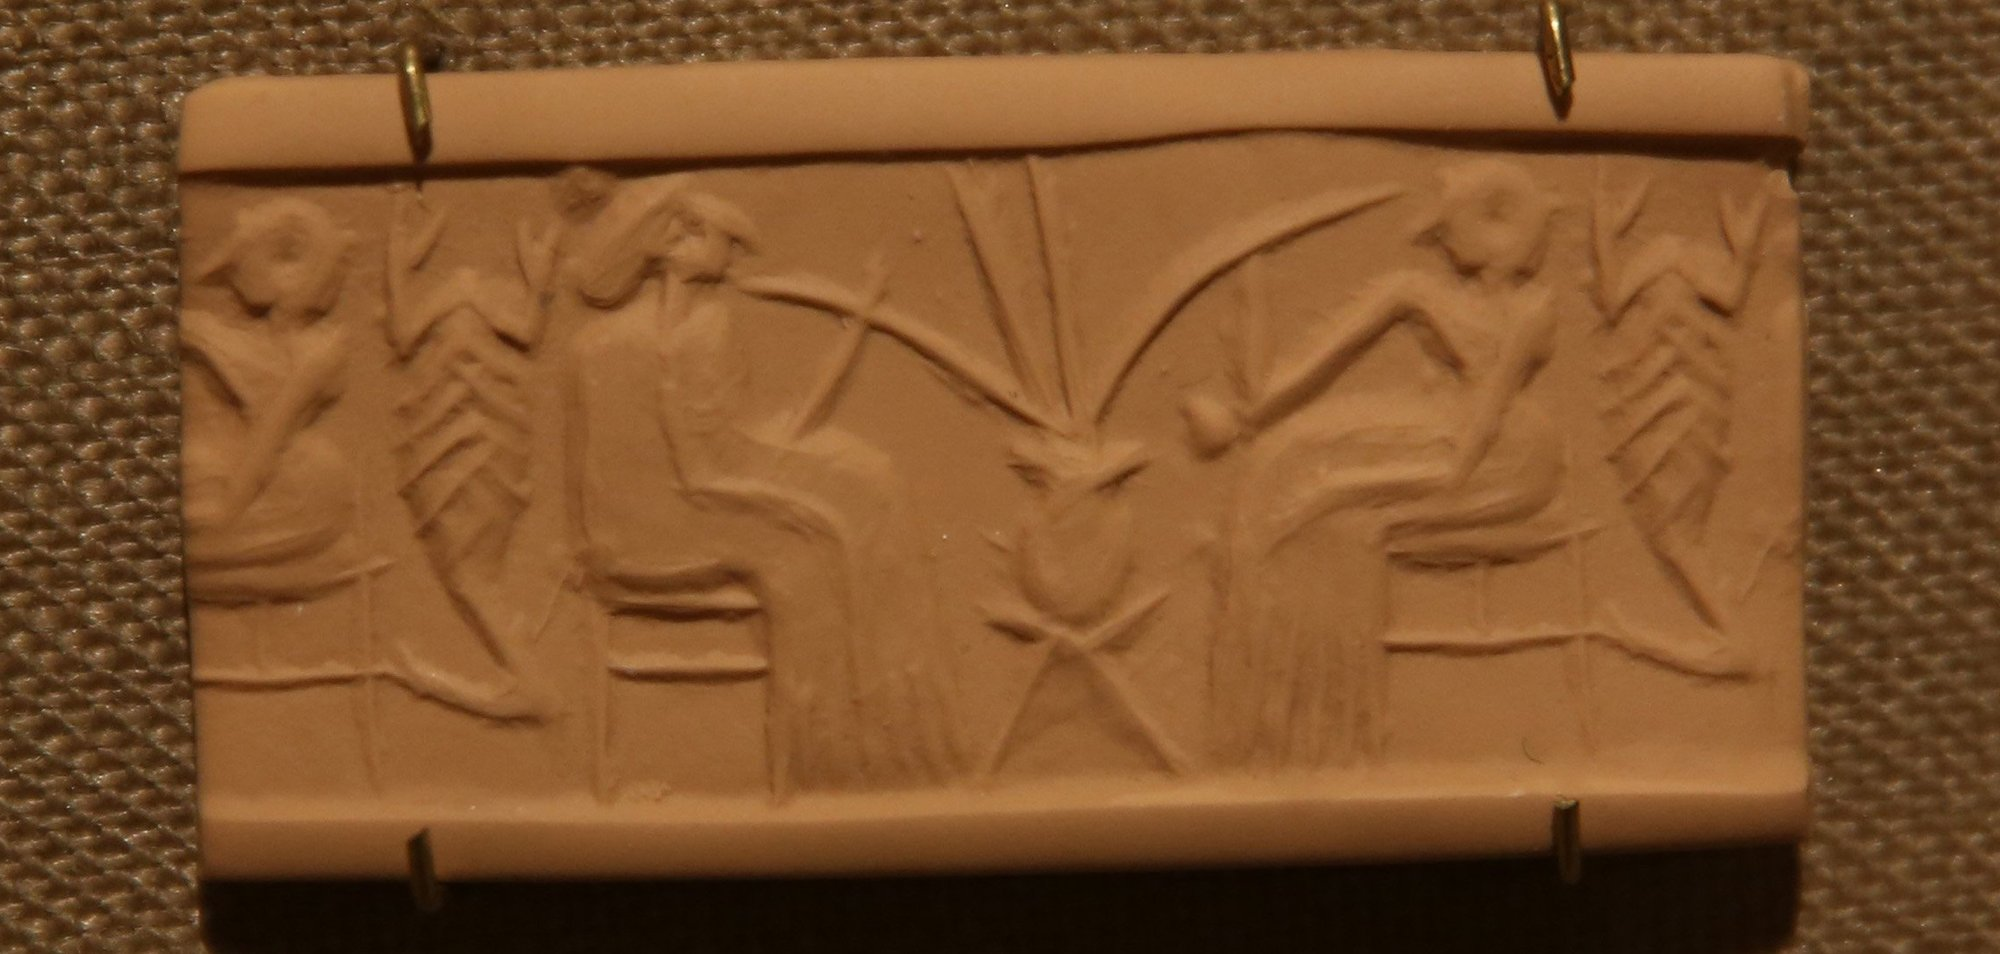
\includegraphics[width=\textwidth]{sumerian.jpg}
\end{frame}

\section{Ingredients}
\againframe<2>{agenda}
\begin{frame}
  \frametitle{Malt}
  \begin{overprint}
    \onslide<1>Germinated barley\\\includegraphics[width=\textwidth]{malt.jpg}
    \onslide<2>Plus sometimes other grains\\\includegraphics[width=\textwidth]{malt.jpg}
    \onslide<3>Or not barley at all\\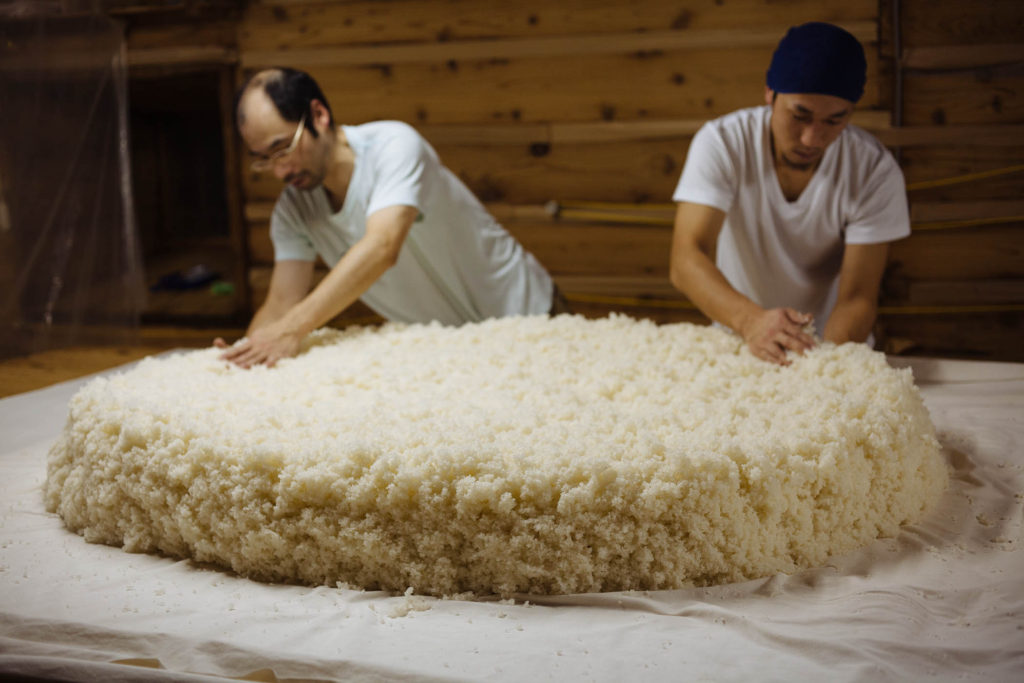
\includegraphics[width=\textwidth]{koji.jpg}
  \end{overprint}
\end{frame}

\begin{frame}
  \frametitle{Hops}
    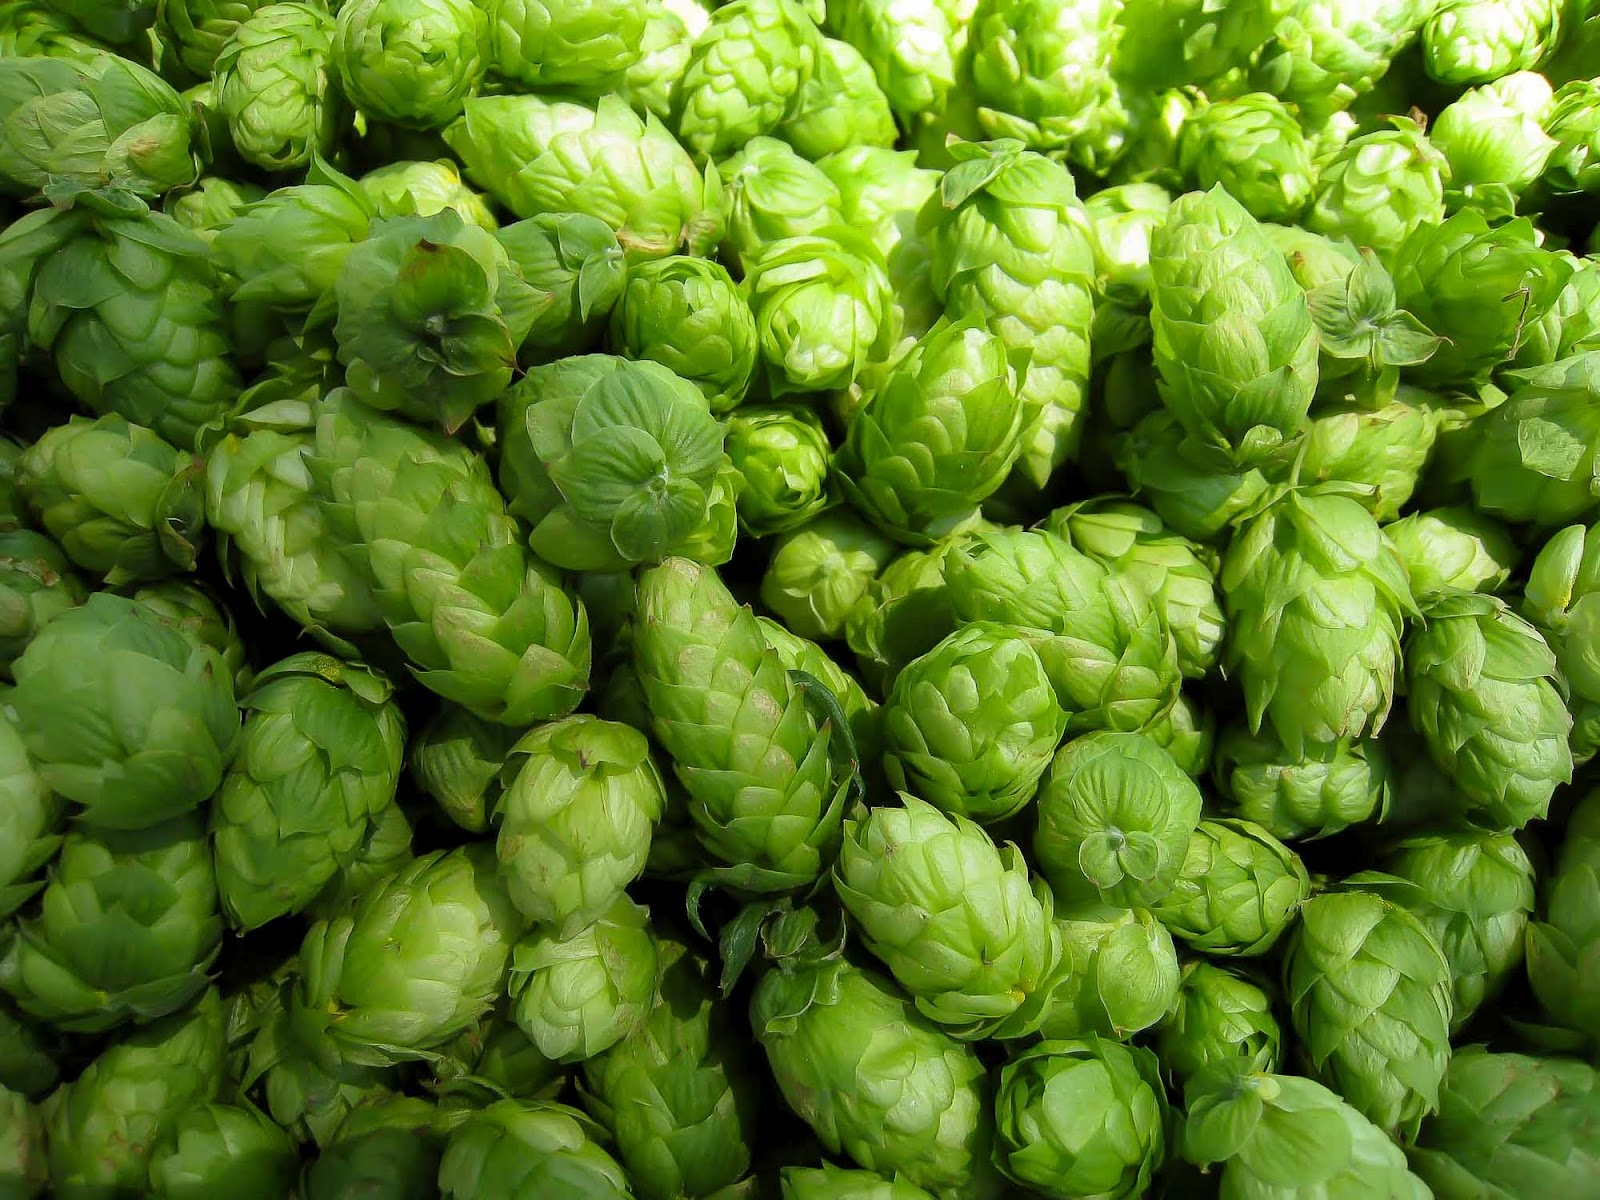
\includegraphics[width=\textwidth]{hops.jpg}
\end{frame}

\begin{frame}
  \frametitle{Yeast}
    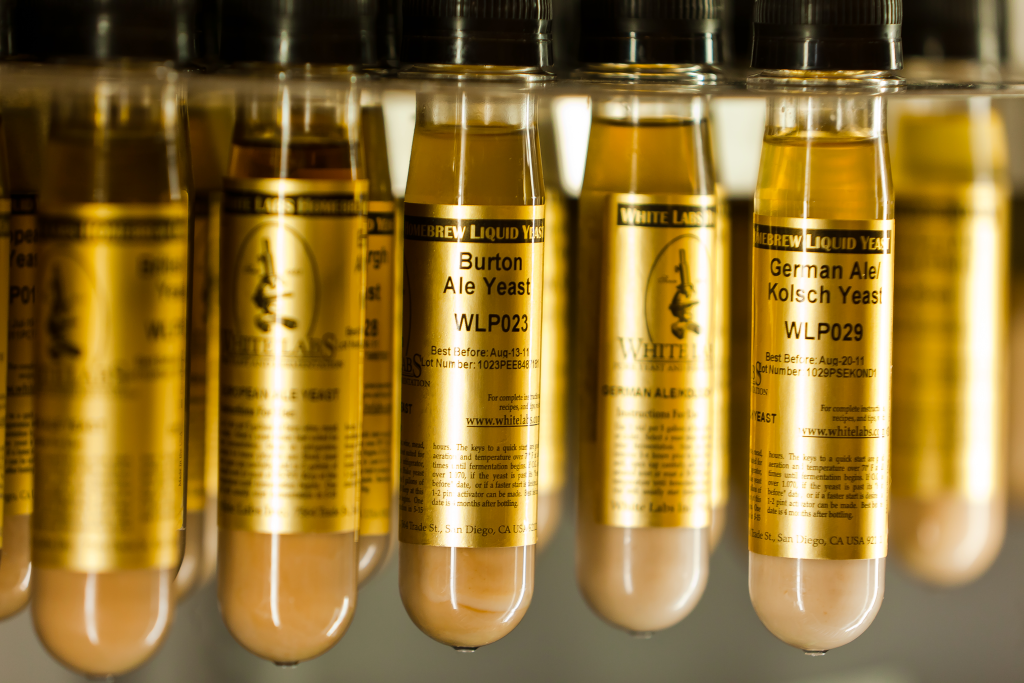
\includegraphics[width=\textwidth]{yeast.png}

\end{frame}

\begin{frame}
  \frametitle{Water}
    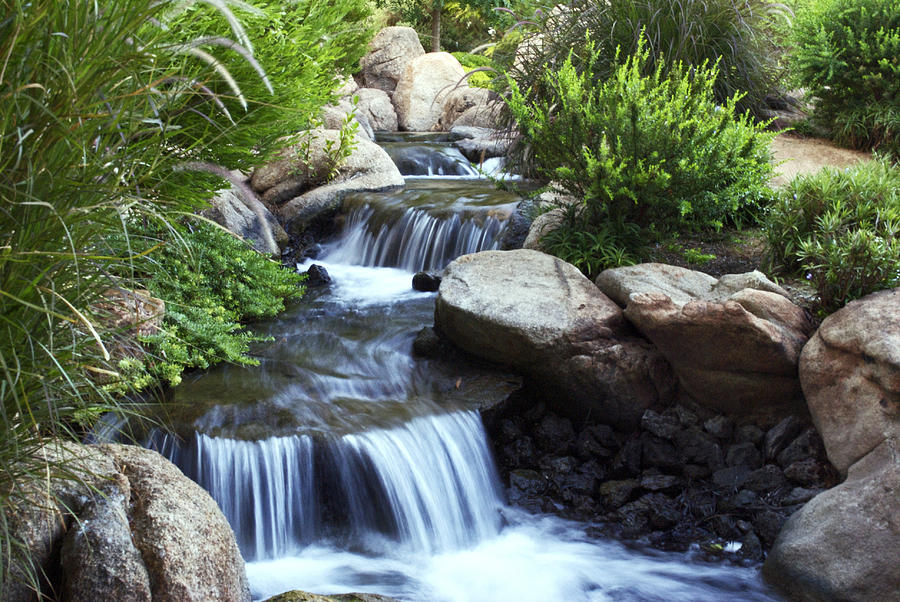
\includegraphics[width=\textwidth]{water.jpg}

\end{frame}

\section{Process}
\againframe<3>{agenda}
\begin{frame}<1-2>[label=diag]
  \frametitle{Commercial brewing}
  \begin{overprint}
    \onslide<1>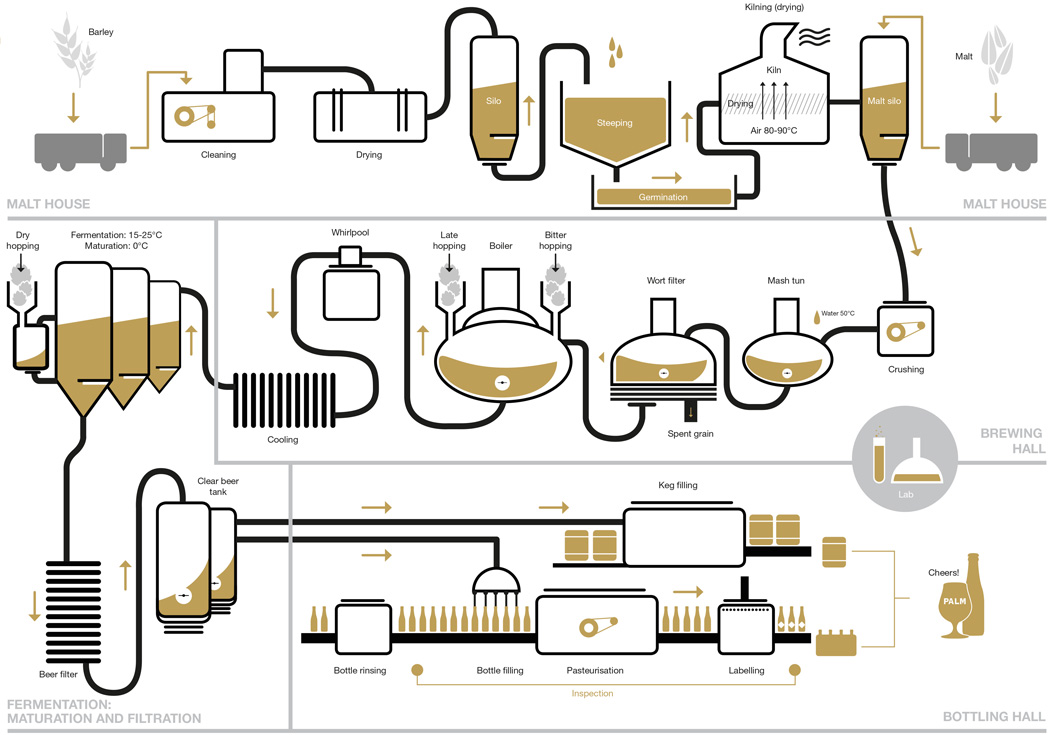
\includegraphics[width=\textwidth]{beerprocess.jpg}
    \onslide<2->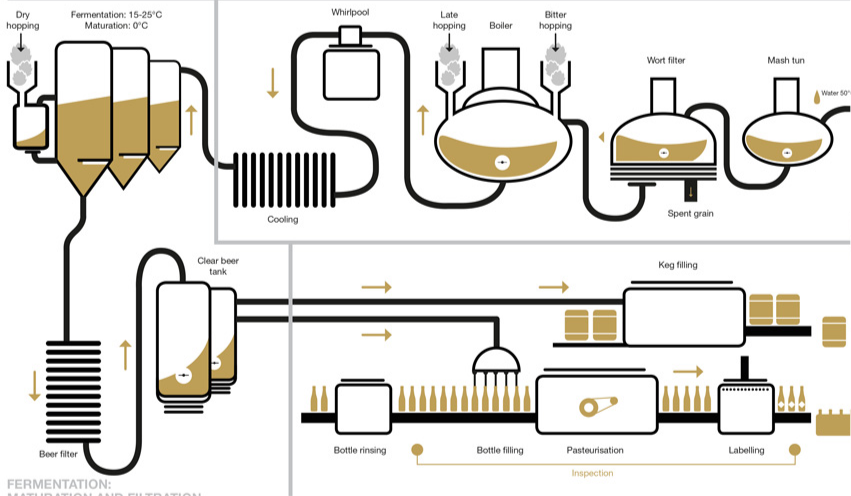
\includegraphics[width=\textwidth]{beerprocesszoom.png}\\
  \end{overprint}
\end{frame}

\begin{frame}
  \frametitle{Mashing chemistry}
  \begin{overprint}
    \onslide<1>\centering 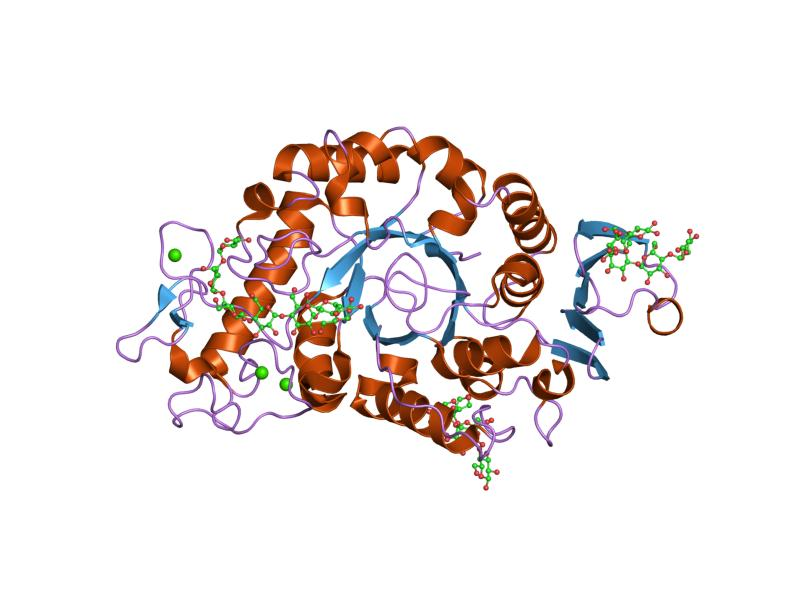
\includegraphics[height=0.8\textheight]{amylase.jpg}\hbox{\textgreek{α}-amylase}\\
    \onslide<2>\centering amylose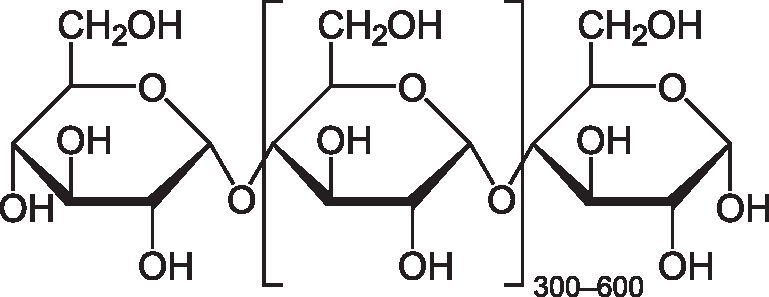
\includegraphics[width=0.8\textwidth]{amylose.pdf}\\
    \onslide<3>\centering dextrin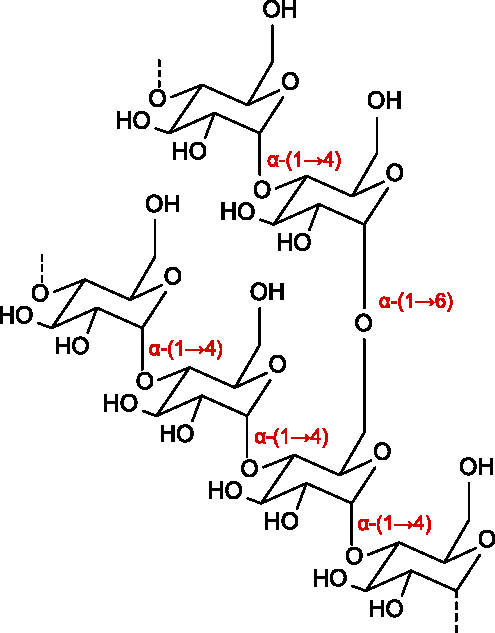
\includegraphics[height=0.8\textheight]{dextrin.pdf}\\
    \onslide<4>\centering maltose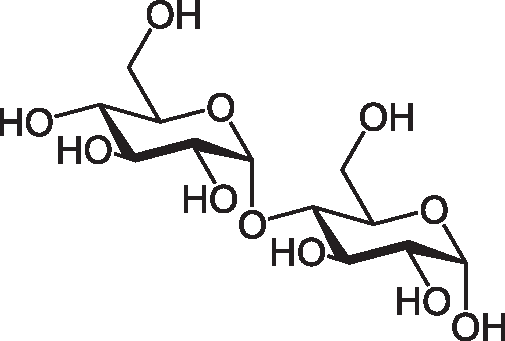
\includegraphics[height=0.4\textheight]{maltose.pdf}\\
  \end{overprint}
\end{frame}

\againframe<2>{diag}

\begin{frame}
  \frametitle{Home-brewing methods}
  \begin{enumerate}
  \uncover<2->{\item All-Grain}
  \uncover<3->{\item Malt extract/brew-in-the-bag}
  \uncover<4->{\item Instant extract kit}
  \end{enumerate}
\end{frame}

\note{Lagering/conditioning}
\note{Priming}

\section{Equipment}
\againframe<4>{agenda}

\begin{frame}<1-2>[label=equip]
  \frametitle{Equipment}
  \begin{enumerate}
  \item\uncover<10->{(Water Treatment)}
  \item\uncover<7->{\alert<7>{Mashing}}
  \item\uncover<10->{\alert<11>{Sparging}}
  \item\uncover<7->{\alert<8>{Boiling}}
  \item\uncover<7->{\alert<9>{Cooling}}
  \item\alert<2>{Primary Fermentation}
  \item\uncover<10->{\alert<12>{Secondary Fermentation}}
  \item\alert<3>{Packaging}\\\bigskip
  \item\alert<4>{Sanitation}
  \item\alert<5>{Measurement \& Miscellanous}
  \end{enumerate}
\end{frame}

\begin{frame}
  \frametitle{Fermentation vessels}
  \begin{itemize}
  \item Plastic bucket
  \onslide<2->\item Carboy/demijohn
  \onslide<3->\item Fancy temperature-controlled steel cone
  \end{itemize}
\end{frame}

\againframe<3-5>{equip}
\begin{frame}
  \frametitle{Measurement \&c.}
  \begin{itemize}
  \item Thermometer
  \item Hydrometer
  \item Scale
    \onslide<2->\item Water chemistry
    \item Pressure gauge
    \item Hop spider
    \item Filter bag
    \item Bottle capper
    \item Siphon
  \end{itemize} 
\end{frame}

\againframe<6-7>{equip}
\begin{frame}
  \frametitle{Mashing}
  \begin{itemize}
  \item Saucepan
  \onslide<2->\item Insulated vessel
  \onslide<3->\item Insulated + heating element (dedicated mash tun)
  \end{itemize}
\end{frame}

\againframe<8>{equip}
\begin{frame}
  \frametitle{Boiling}
  \begin{itemize}
  \item Saucepan(s)
  \onslide<2->\item Boiler
  \onslide<3->\item All-in-one
  \end{itemize}
  
\end{frame}
\begin{frame}
  \frametitle{Otto}
  \begin{center}
    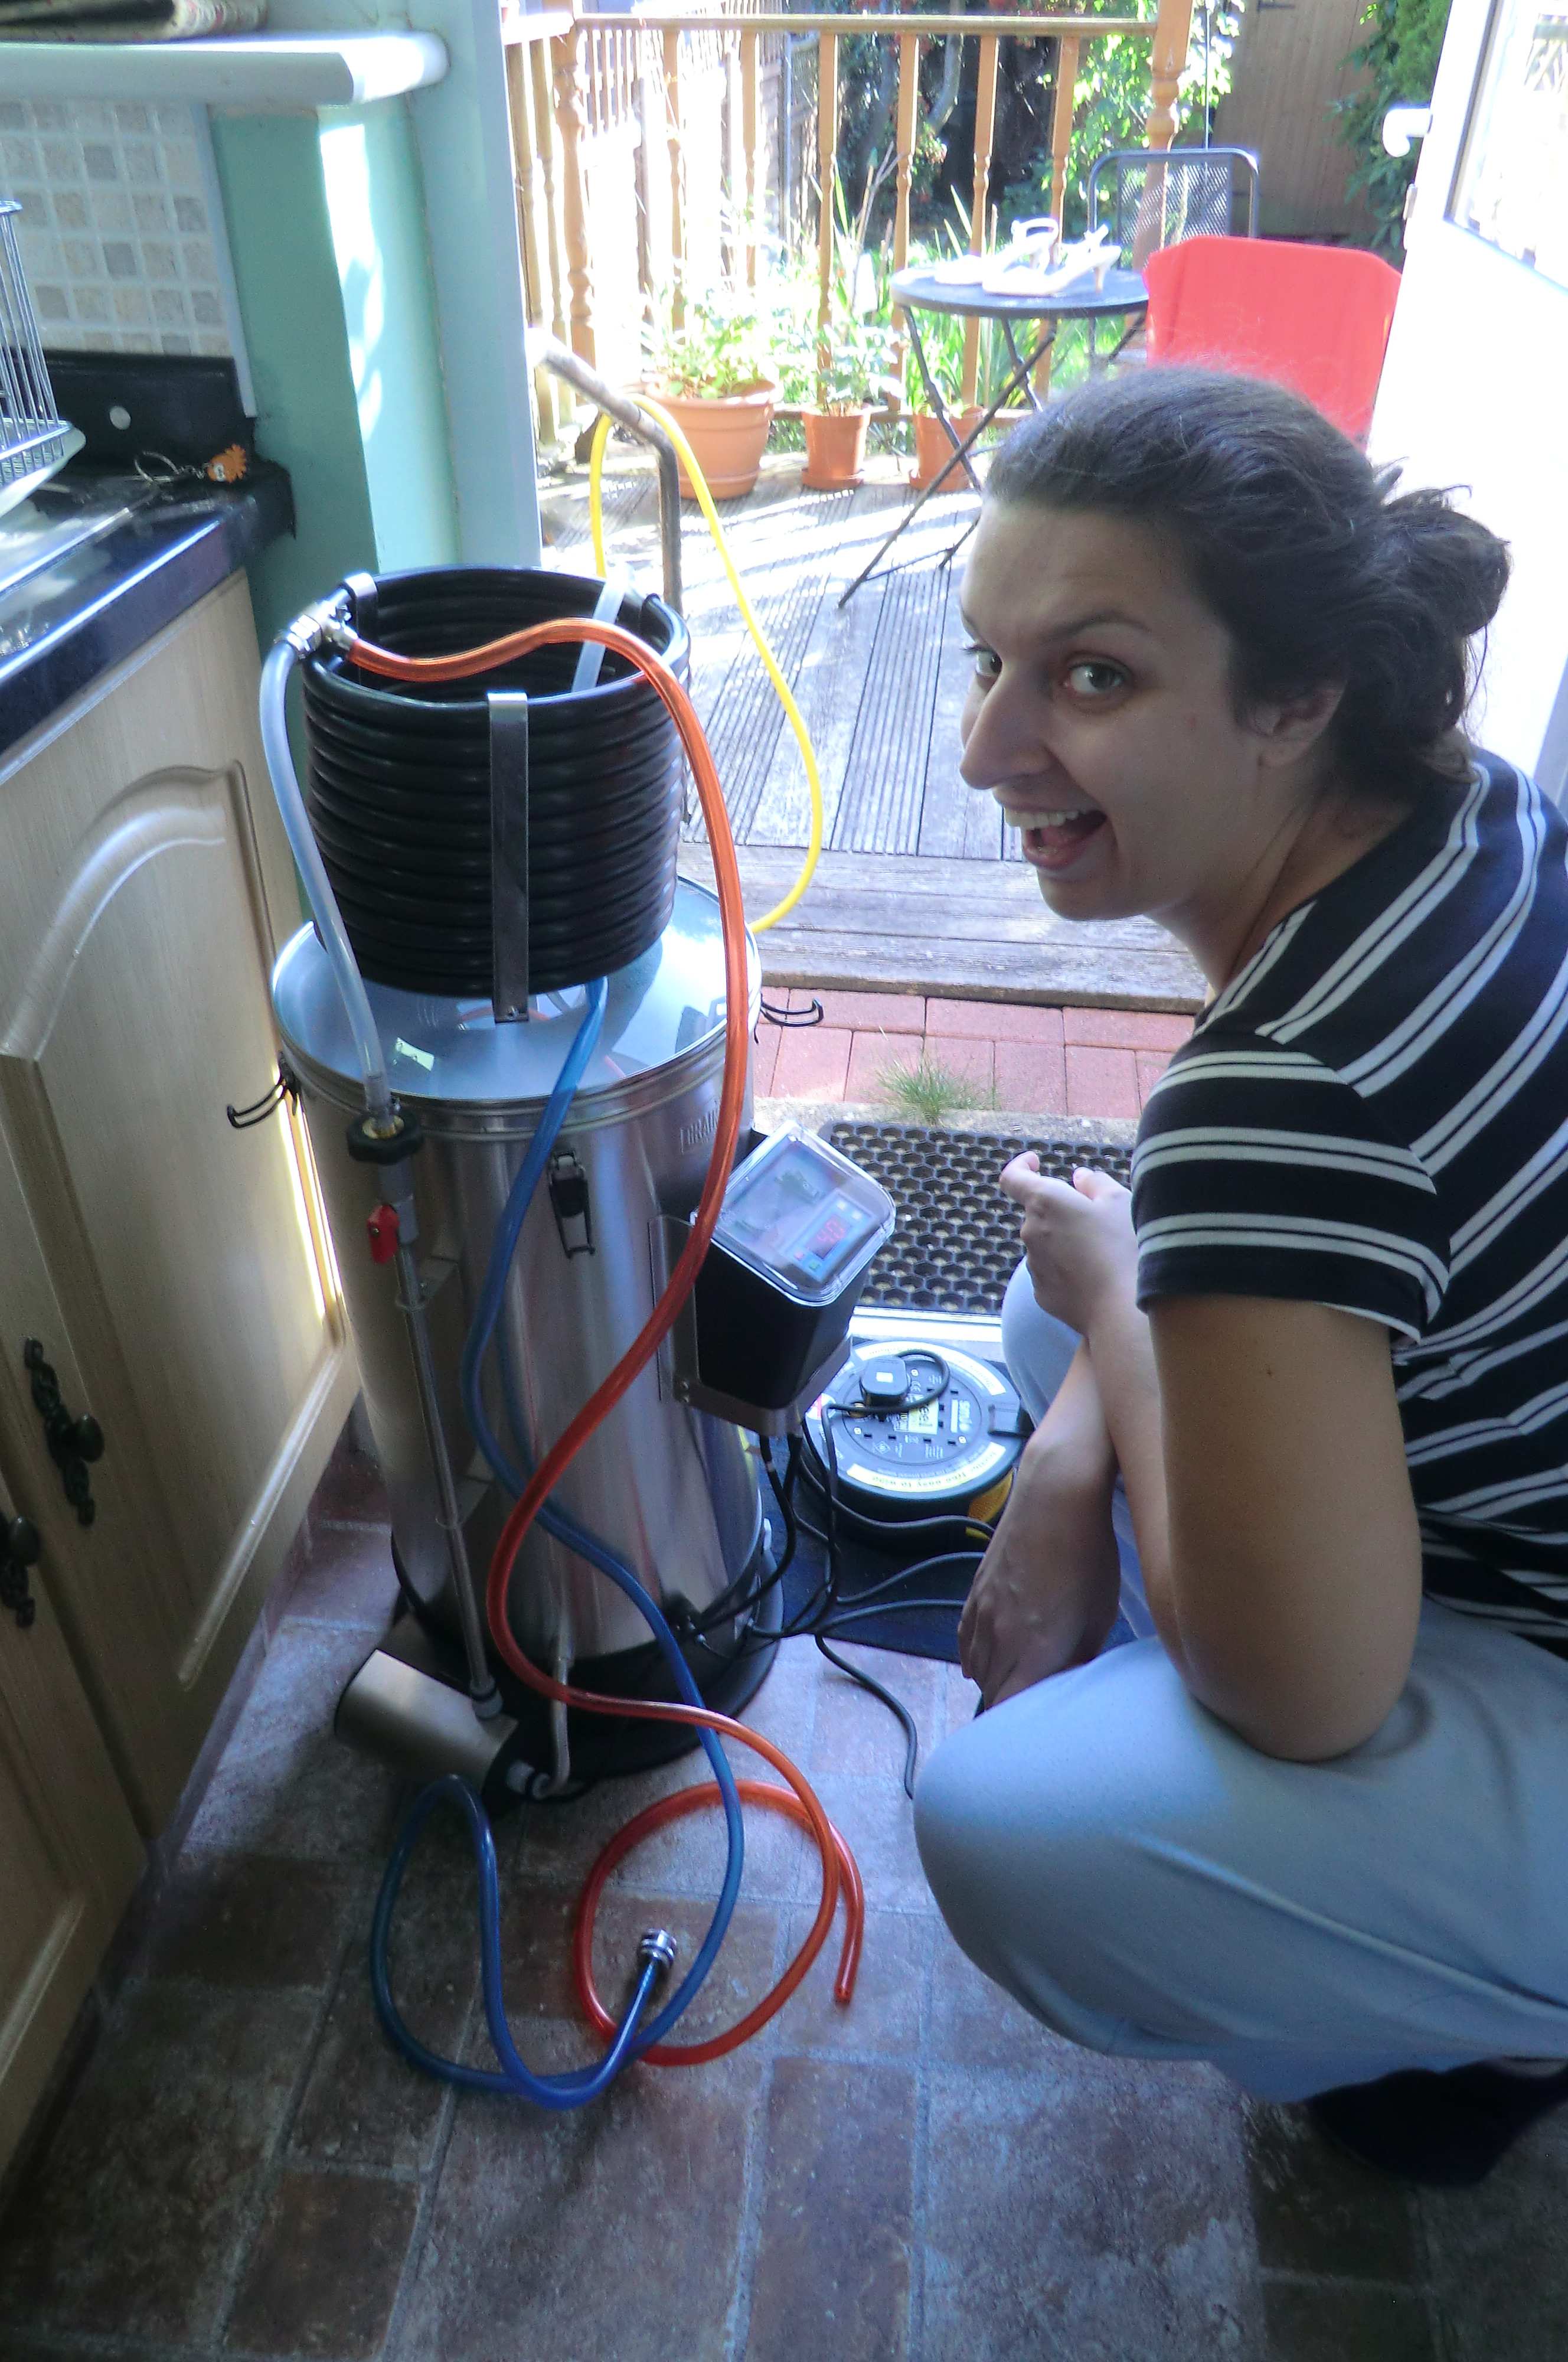
\includegraphics[height=0.9\textheight]{CIMG2985.JPG}
  \end{center}
\end{frame}

\againframe<9-11>{equip}
\begin{frame}
  \frametitle{Sparging}
  \begin{itemize}
  \item Nothing
  \onslide<2->\item Bag sparging
  \onslide<3->\item Remashing
  \onslide<4->\item Fly sparging
  \end{itemize}
  
\end{frame}

\againframe<12>{equip}

\section{Economics}
\againframe<5>{agenda}

\begin{frame}{Ingredients costs}
  (Based on batch size of 23l)\\
  Instant kit: \like £30/batch=£1300/kl\\\bigskip
  \onslide<2-> Grist: £5--9\\
  Hops: £1--3\\
  Yeast: £2--12\\
  \onslide<3-> Electricity: \like 6--7kWh\\
  Water: \like 60l\\
  \onslide<4-> Total: \like £11/batch=£470/kl
\end{frame}

\begin{frame}
  \frametitle{Equipment costs}
  Setup \textsc{i}: bare-bones\\
  \onslide<2->FV: \like £20, lasts 60 brews\\
  \onslide<3-> Measuring and miscellaneous: \like £30\\
  \onslide<4-> Upfront: \like £50\\
  \onslide<5-> Amortized: \like £0.5/batch=£21/kl
\end{frame}

\begin{frame}
  \frametitle{Equipment costs}
  Setup \textsc{ii}: basic full-mash\\
  \onslide<2-> Mash tun: \like £100, lasts 120 brews\\
  \onslide<3-> Boiler: \like £90, lasts 120 brews\\
  \onslide<4-> FV: \like £20, lasts 60 brews\\
  \onslide<5-> Cooling: Home-made or improvised? £10?\\
  \onslide<6-> Measuring and miscellaneous: \like £30\\
  \onslide<7-> Upfront: \like £260\\
  \onslide<8-> Amortized: \like £2/batch=£83/kl
\end{frame}

\begin{frame}
  \frametitle{Equipment costs}
  Setup \textsc{iii}: Grainfather\\
  \onslide<2-> All-in-one mash tun, boiler, chiller: \like £675\\
  \onslide<3-> FV: \like £20, lasts 60 brews\\
  \onslide<4-> Measuring and miscellaneous: \like £30\\
  \onslide<5-> Upfront: \like £750\\
  \onslide<6-> Amortized: \like £5/batch=£220/kl\\\bigskip
  \onslide<7-> (Or scale up to 50l for \like £2200)
\end{frame}

\begin{frame}
  \frametitle{Equipment costs}
  Setup \textsc{iv}: Fancy higher-scale\\
  \onslide<2-> 75l Mash tun: £465\\
  \onslide<3-> 120l Boiler: £480\\
  \onslide<4-> 155l Fermenter: £1200
\end{frame}

\begin{frame}
  \frametitle{Packaging costs}
  \onslide<1-> PET bottles: \like £0.41, reusable 3--4 times\\
  \onslide<2-> Reuse bottles you've bought (1l mixers, beer)\\
  \onslide<3-> Glass bottles: \like £0.80, reusable 6--8 times\\
  \onslide<4-> Barrel: \like £30 (not recommended)\\
  \onslide<5-> 18 l keg system: \like £150
\end{frame}

\section{Pitfalls}
\againframe<6>{agenda}
\begin{frame}
  \frametitle{Pitfalls}
  \begin{itemize}
   
    \onslide<1->\item Cleanliness\\
    \onslide<2->\item Yeast health\\
    \onslide<3->\item Mashing temperature control\\
    \onslide<4->\item Fermentation temperature control\\
    \onslide<5->\item Bottle bombs\\
    \onslide<6->\item Bad record-keeping\\
    \onslide<7->\item Recipe mistakes\\
    \onslide<8->\item Physical mistakes
  \end{itemize}
\end{frame}

\section{Recipe design}
\againframe<7>{agenda}
\begin{frame}
  \frametitle{Recipe design}
    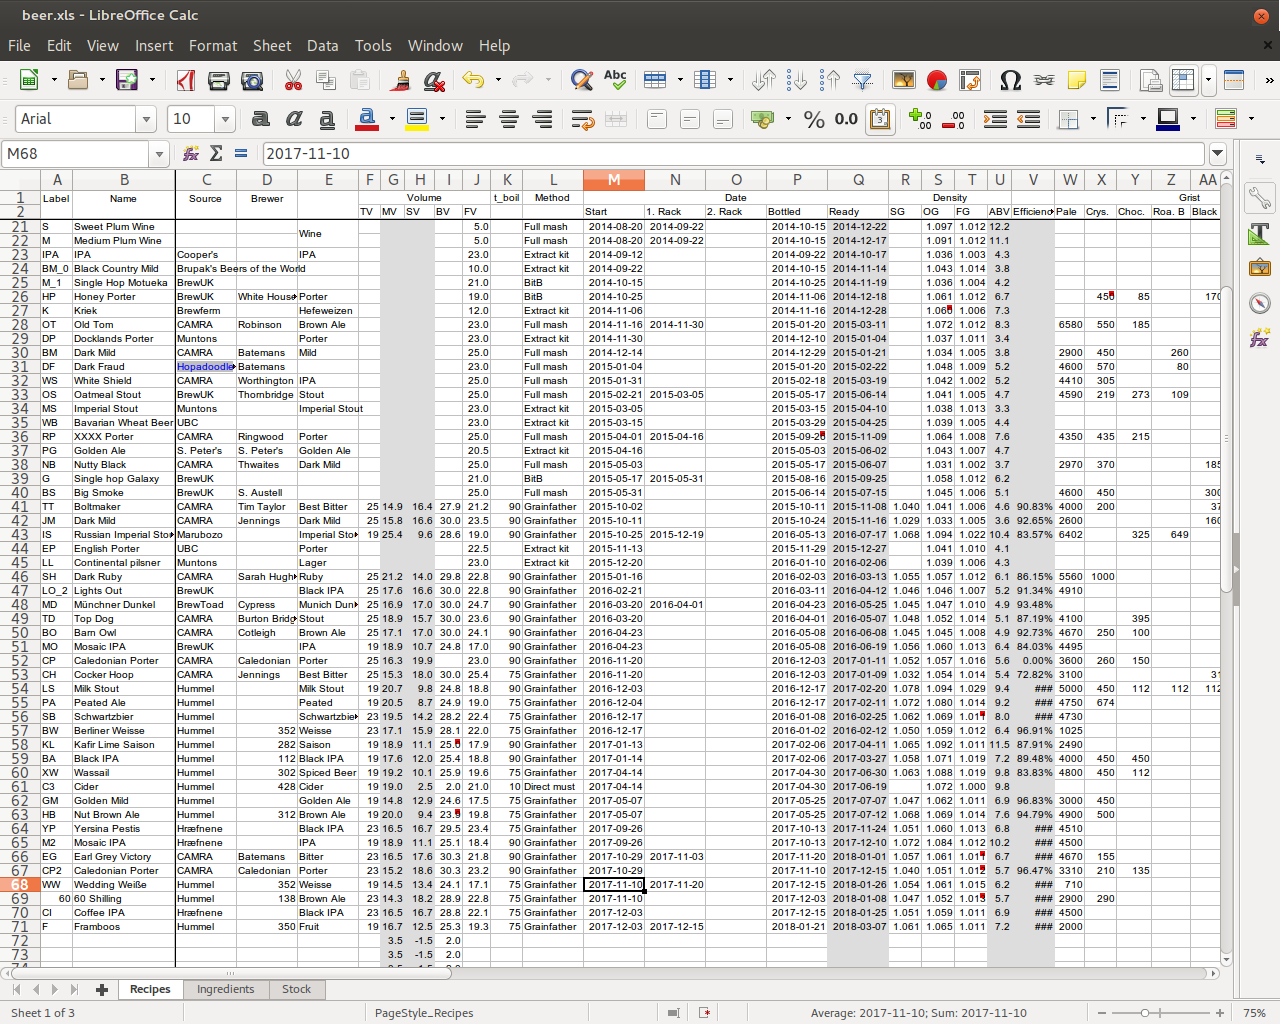
\includegraphics[width=\textwidth]{xls.png}
\end{frame}

\begin{frame}
  \frametitle{Grist}
  \begin{itemize}
  \item Base malts
    \begin{itemize}
    \item Maris Otter, Wheat malt, Pilsner malt, Vienna malt\ldots{}
    \end{itemize}
  \item Roasted malts
    \begin{itemize}
    \item Chocolate malt, black malt\ldots{}
    \end{itemize}
  \item Caramelized malts
    \begin{itemize}
    \item Carafa, Crystal malts, Caramalt\ldots{}
    \end{itemize}
  \item Weird malts
    \begin{itemize}
    \item Rauchmalz, peated malt\ldots{}
    \end{itemize}
    \bigskip
  \item Adjuncts
    \begin{itemize}
    \item Torrified wheat, roasted barley, dextrose, honey\ldots
    \end{itemize}
  \item Other grains
    \begin{itemize}
    \item Rye, sorghum, rice, corn\ldots
    \end{itemize}

  \end{itemize}
\end{frame}

\begin{frame}
  \frametitle{Hops \& Yeast}
  \begin{itemize}
  \item Bittering hops
  \item Flavour hops
  \item Dry hopping
    \bigskip
  \item Yeast strains
    \begin{itemize}
    \item Mainly \emph{Saccharomyces cerevisi\ae{}}
    \item \emph{Saccharomyces pastorianus}, \emph{S. eubayanus}, \emph{S. carlsbergensis}
    \item \emph{Brettanomyces bruxellensis}
    \end{itemize}
  \item Bacterial cultures
    \begin{itemize}
    \item \emph{Lactobacillus}, \emph{Pediococcus}\ldots
    \end{itemize}
  \item Wild yeast
    \bigskip
  \item Racking, lagering, conditioning
\end{itemize}
\end{frame}

\begin{frame}
  \frametitle{Flavourings \& Additives}
  \begin{itemize}
  \item Finings \& Body
    \begin{itemize}
    \item Isinglass, Irish moss, maltodextrin, lactose\ldots
    \end{itemize}
  \item Fruit
  \item Nuts \& Spices
    \begin{itemize}
    \item Hazelnut
    \item Cardamom
    \item Coriander
    \item Chili
    \item Juniper
    \end{itemize}
  \item Coffee
  \item Resin \& bark
  \item Chocolate
  \item Wood chips and barrel aging
\end{itemize}

\end{frame}

\begin{frame}[label=summary]
  \frametitle{Summary}
  \begin{itemize}
  \item You can improvise
  \item You can find loads of recipes
  \item \ldots{} or make them up
  \item The startup costs needn't be too bad
  \item You will get more out of drinking beer
\end{itemize}
\end{frame}

\begin{frame}
  \frametitle{Research}
  \begin{center}
    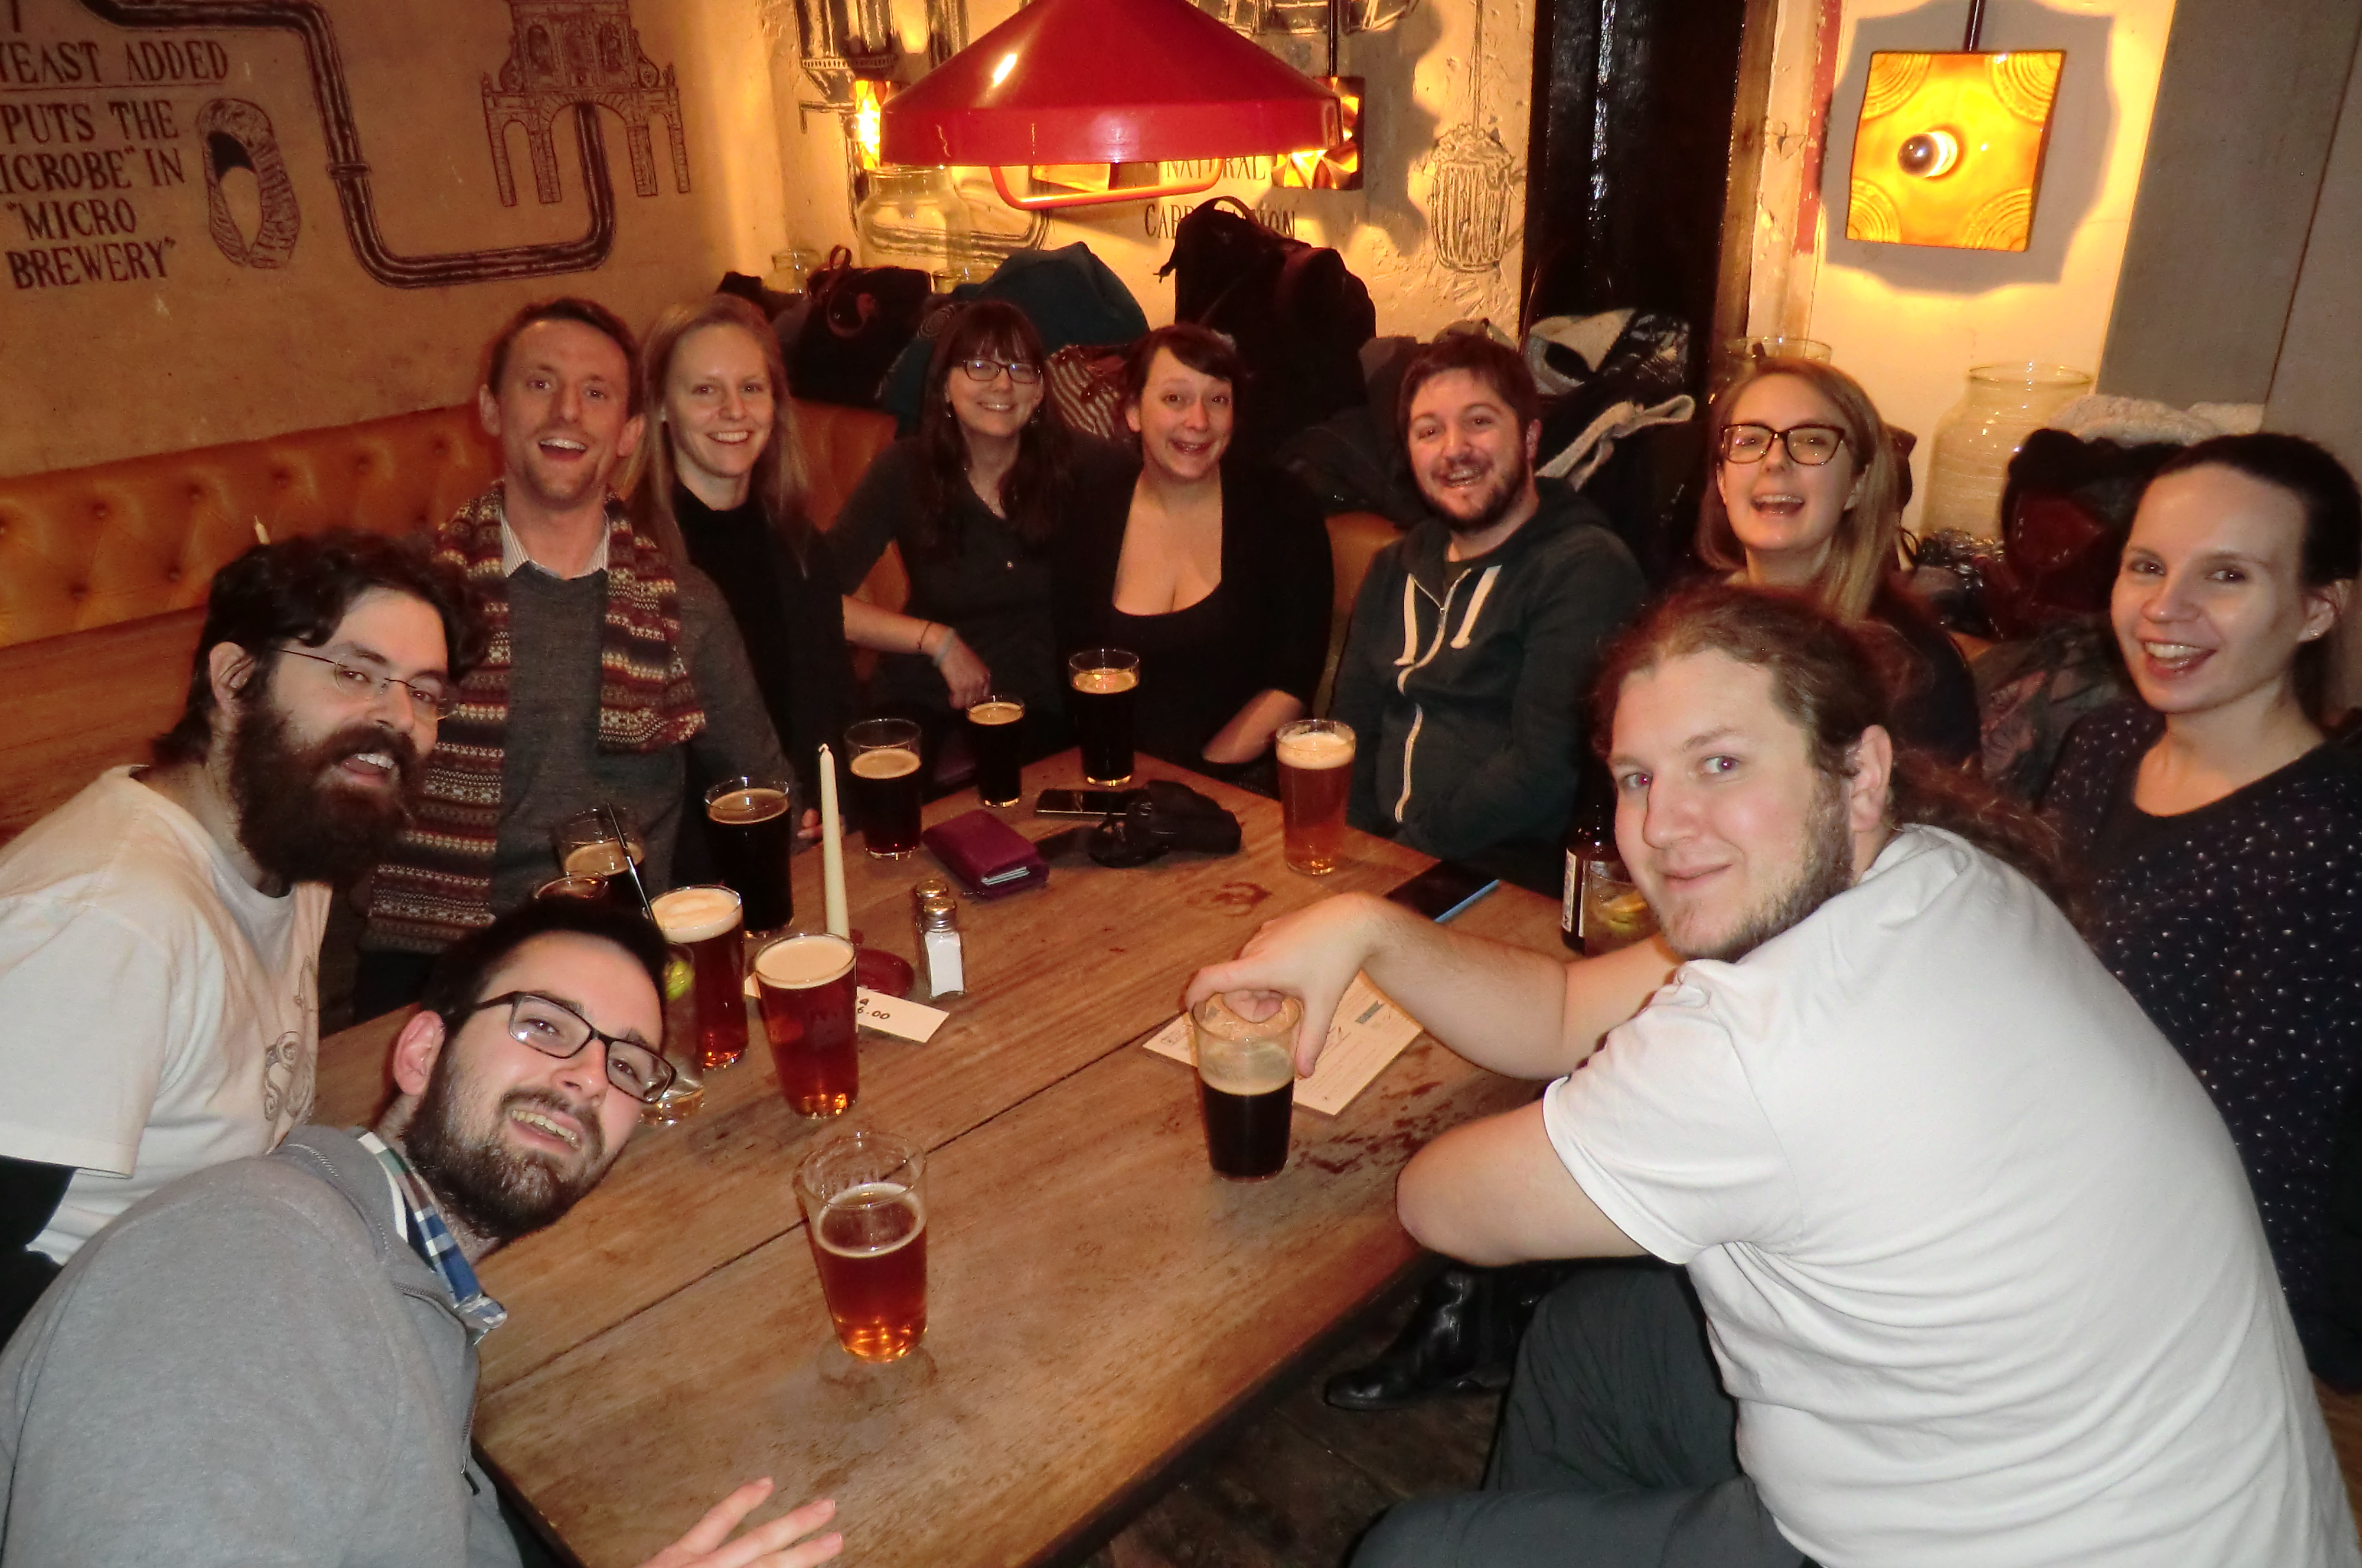
\includegraphics[height=0.9\textheight]{CIMG4062.JPG}
  \end{center}
\end{frame}

\section{Resources}
\againframe<8>{agenda}
\begin{frame}{Resources}
  Books
  \begin{itemize}
  \item \href{http://www.howtobrew.com/}{Palmer, \emph{How to Brew} (1st ed.\ free online)}
  \item
    \href{https://www.goodreads.com/book/show/11095467-the-complete-homebrew-beer-book}{Hummel, \emph{The Complete Homebrew Book}}
  \item \href{https://shop.camra.org.uk/brew-your-own-british-real-ale.html}{\emph{CAMRA's Brew your own British Real Ale}}
  \end{itemize}
  
  Blogs, fora, calculators
  \begin{itemize}
  \item\href{https://www.brewersfriend.com/stats/}{Brewer's Friend Calculators}
  \item\href{https://www.homebrewtalk.com/forum/}{Homebrew Talk}
  \item\href{https://www.homebrewersassociation.org/homebrew-recipes/}{American Homebrewers Association}
  \item\href{http://beersmith.com/beer-recipes/}{BeerSmith}
  \end{itemize}
  (Links are live in the slide deck)
\end{frame}

\begin{frame}
  \frametitle{Thanks!}
  Questions?
\end{frame}
\end{document}

%%% Local Variables:
%%% mode: latex
%%% TeX-master: "brewing"
%%% End: